\chapter{Tips in DL}

\section{Enlarge the FOV}

增加网络的感受野。目前看到的主要方法如下:

\begin{itemize}
\item CRFs\cite{marvin2018crf}
\item Global Graph-reasoning module\cite{chen18iterative}
\item Pooling
\item Dilated conv\cite{YuKoltun2016}
\item 
\end{itemize}


\section{Upsampling}

在卷积以及Pooling之后保持分辨率。目前看到的主要方法如下:

\begin{itemize}
\item Padding
\item Deconvolution
\item Uppooling
\item Bilinear
\item 
\end{itemize}


\section{Multiscale Ability}

在目标检测(Object Detection)中加入多尺度信息。记得的有以下几个方法:

\begin{itemize}
\item Pyramid Network
\item Stacked CNN ?
\item 
\end{itemize}


\section{Dilated Convolution}

主要原理如下。

\begin{figure}[!hbtp]
\centering
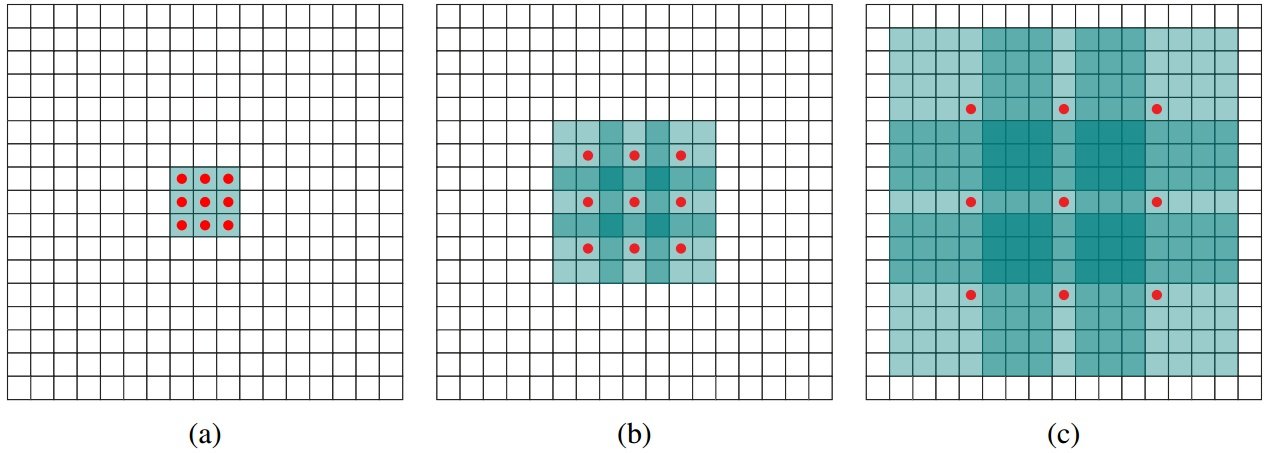
\includegraphics[width=0.75\textwidth]{DLTips/DilatedConv1}
\caption{Dilated Convolution示意图}
\label{DilatedConv1}
\end{figure}

{\bfseries 注意,下文提到的N-Dilated Conv中的$N={1, 2, 3, \ldots}$是指图中相邻红点之间的间隔。}

图\ref{DilatedConv1}中,(a)图对应3x3的1-dilated conv,和普通的卷积操作一样,(b)图对应3x3的2-dilated conv,实际的卷积kernel size还是3x3,但是空洞为1,也就是对于一个7x7的图像patch,只有9个红色的点和3x3的kernel发生卷积操作,其余的点略过。也可以理解为kernel的size为7x7,但是只有图中的9个点的权重不为0,其余都为0。 可以看到虽然kernel size只有3x3,但是这个卷积的感受野已经增大到了7x7{\bfseries(如果考虑到这个2-dilated conv的前一层是一个1-dilated conv的话,那么每个红点就是1-dilated的卷积输出,所以感受野为3x3,所以1-dilated和2-dilated合起来就能达到7x7的conv)},(c)图是4-dilated conv操作,同理跟在两个1-dilated和2-dilated conv的后面,能达到15x15的感受野。对比传统的conv操作,3层3x3的卷积加起来,stride为1的话,只能达到(kernel-1)*layer+1=7的感受野,也就是和层数layer成线性关系,而dilated conv的感受野是指数级的增长。

Dilated的好处是不做Pooling算是信息的情况下,加大了感受野,让每个卷积核输出都包含较大范围的信息。在图像需要全局信息或者语音文本需要较长的Sequence信息依赖的问题中,都能很好的应用Dilated Convolution, 比如图像分割、语音合成WaveNet、机器翻译ByteNet。

WaveNet的例子。
\begin{figure}[!hbtp]
\centering
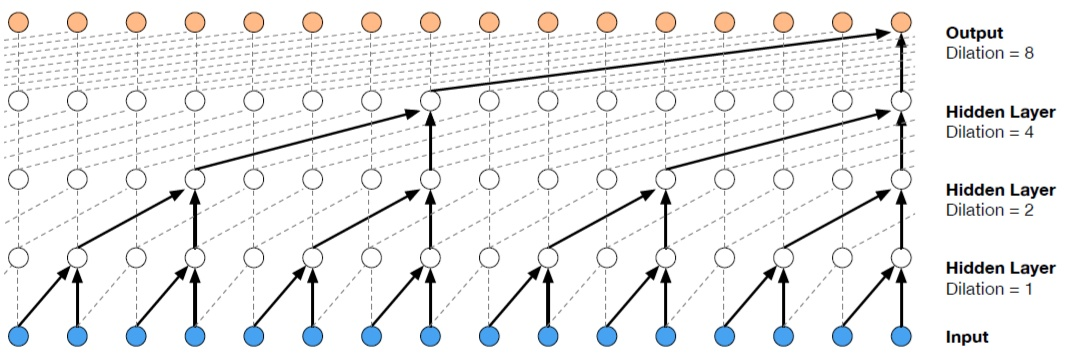
\includegraphics[width=0.75\textwidth]{DLTips/WaveNet1}
\caption{Dilated Convolution在WaveNet中的应用示意图}
\label{WaveNet1}
\end{figure}

参考文献:\href{https://www.zhihu.com/search?type=content\&q=dilated\%20CNN}{Dilated Conv 知乎}

\section{Deconvolutional Network}

务必看\textbf{补充}部分的内容!

参考文献:\href{https://www.zhihu.com/question/43609045/answer/132235276}{Deconvolution Networks}

可能应用的领域:Visualization, Pixel-wise Prediction, Unsupervised Learning, Image Generation.

大致可分为以下几个方面:
\begin{itemize}
\item Unsupervised Learning 

其实是 Covolutional Sparse Coding. 这里的Deconv只是观念上和传统的Conv反向,传统的conv是从图片生成feature map,而deconv是用unsupervised的方法找到一组kernel和feature map,让它们重建图片。

\item CNN Visualization

通过deconv将CNN中conv得到的feature map还原到像素空间,以观察特定的feature map对哪些pattern的图片敏感,这里的deconv其实不是conv的可逆运算,只是conv的transpose,所以tensorflow里一般取名叫transpose\_conv。

\item Upsampling

在pixel-wise prediction比如image segmentation[4]以及image generation[5]中,由于需要做原始图片尺寸空间的预测,而卷积由于stride往往会降低图片size, 所以往往需要通过upsampling的方法来还原到原始图片尺寸,deconv就充当了一个upsampling的角色。

\end{itemize}

下面主要介绍这三个方面的论文。

\subsection{Convolutional Spare Coding}

{\bfseries 第一篇:Deconvolutional Netwoks}

主要用于学习图片的中低层级的特征表示,属于Unspervised Feature Learning。

更多内容参考本小节的参考文献。

\subsection{CNN可视化}
ZF-Net中利用Deconv来做可视化,它是将CNN学习到的Feature Map的卷积核,取转置,将图片特征从Feature Map空间转化到Pixel空间,用于发现哪些Pixel激活了特定的Feature Map,达到分析理解CNN的目的。


\subsection{Upsampling}
用于FCN\cite{Fcn2014}和DCGAN。

\subsection{补充}

{\bfseries 一个非常好的可以看到多种卷积操作动作图的资源:}\href{https://github.com/vdumoulin/conv_arithmetic}{Convolution Arithmetic Github}


上面的东西还是没有说明白Deconvolution到底是怎么回事啊。

\begin{quote}
实际使用中,反卷积会引起棋盘状的Artifacts。所以要采用上采样卷积层。
\end{quote}
上面这句话是什么意思?

\subsection{Deconvolution与Upsample的区别}

参考文献:\href{https://www.zhihu.com/question/63890195}{Caffe中的Deconvolution和Upsample区别-知乎}

高票回答:

Deconvolution

\begin{figure}[!htbp]
\centering
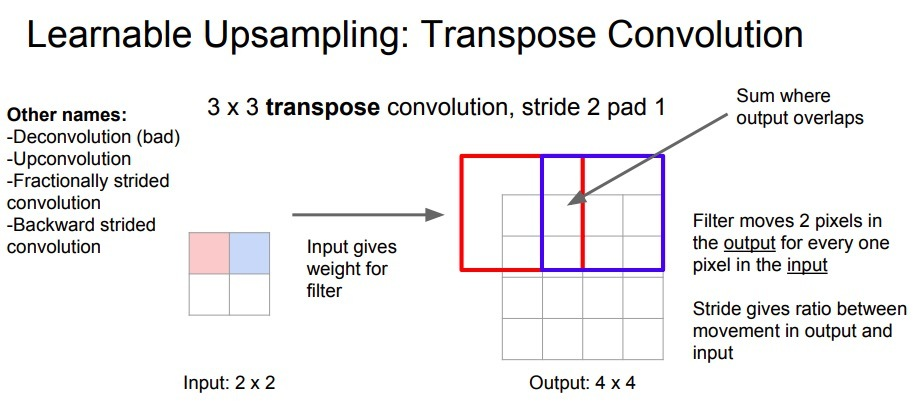
\includegraphics[width=0.75\textwidth]{DLTips/Deconvolution0.jpg}
\caption{Transpose Convolution过程示意图}
\label{Deconvolution0}
\end{figure}

Input pixel * filter = output window,不同output window重合的部分使用sum叠加处理。

这一解释和caffe的定义保持一致,caffe中定义解释过来就是:“DeconvolutionLayer 逐像素地将输入值乘上一个filter,并将结果输出windows叠加起来”

Convolve the input with a bank of learned filters, and (optionally) add biases, treating filters and convolution parameters in the opposite sense as ConvolutionLayer.ConvolutionLayer computes each output value by dotting an input window with a filter; DeconvolutionLayer multiplies each input value by a filter elementwise, and sums over the resulting output windows. In other words, DeconvolutionLayer is ConvolutionLayer with the forward and backward passes reversed. DeconvolutionLayer reuses ConvolutionParameter for its parameters, but they take the opposite sense as in ConvolutionLayer (so padding is removed from the output rather than added to the input, and stride results in upsampling rather than downsampling).

Upsampling

该层权重通过BilinearFiller初始化,因此当学习率为0时,权重在训练过程中保持初始值不变,一一直作为bilinear resize的作用。

\lstset{language=Python, caption={Bilinear filter initializer in MXNet}}
\begin{lstlisting}
class Bilinear(Initializer)
"""Initialize weight for upsampling layers."""
def __init__(self):
    super(Bilinear, self).__init__()
def _init_weight(self, _, arr):
    weight = np.zeros(np.prod(arr.shape), dtype='float32')
    shape = arr.shape
    f = np.ceil(shape[3] / 2.)
    c = (2 * f - 1 - f % 2) / (2. * f)
    for i in range(np.prod(shape)):
        x = i % shape[3]
        y = (i / shape[3]) % shape[2]
        weight[i] = (1 - abs(x / f - c)) * (1 - abs(y / f - c))
    arr[:] = weight.reshape(shape)
\end{lstlisting}

James Liu的回答:

\begin{itemize}
\item \textbf{Deconvolution}

上采样就是把$[W,H]$大小的feature map $F_{W,H}$扩大为$[nW,nH]$尺寸大小的$\hat{F}_{nW,nH}$,其中$n$为上采样倍数。那么可以很容易的想到我们可以在扩大的feature map $\hat{F}$上每隔$n$个位置填补原F中对应位置的值。

但是剩余的那些位置怎么办呢?deconv操作是把剩余位置填0,然后这个大feature map过一个conv。

\textbf{所以}:Deconv = 扩大 + 填0 + Convolution

\item \textbf{Upsampling}

插值上采样 = 扩大 + 插值

\end{itemize}

\subsubsection{理解深度学习中的Deconvolution Networks}

参考文献:\href{https://www.zhihu.com/question/43609045}{理解深度学习中的Deconvolution Networks - 知乎}


逆卷积(Deconvolution)比较容易引起误会,转置卷积(Transposed Convolution)是一个更为合适的叫法.

\begin{figure}[!hbtp]
\centering
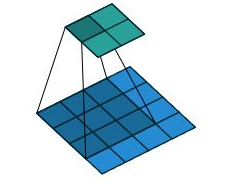
\includegraphics[width=0.5\textwidth]{DLTips/Deconvolution1.png}
\caption{一个例子,用于卷积操作说明}
\label{Deconvolution1}
\end{figure}
输入矩阵可展开为16维向量,记作x

输出矩阵可展开为4维向量,记作y

卷积运算可表示为y = Cx

不难想象C其实就是如下的稀疏阵
\begin{figure}[!htbp]
\centering
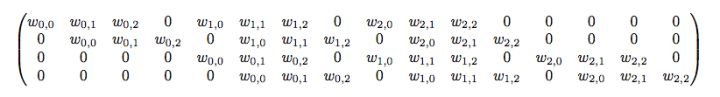
\includegraphics[width=0.5\textwidth]{DLTips/Deconvolution2.jpg}
\caption{卷积操作时的矩阵形式}
\label{Deconvolution2}
\end{figure}

那么当反向传播时又会如何呢?首先我们已经有从更深层的网络中得到的$\frac{\partial Loss}{\partial y}$.

\begin{displaymath}
\frac{\partial{Loss}}{\partial{x_j}} = \sum_{i}\frac{\partial{Loss}}{\partial y_i} \frac{\partial y_i}{\partial{x_j}} = \sum_{i} \frac{\partial{Loss}}{\partial y_i} C_{i, j} = \frac{\partial{Loss}}{y} \cdot C_{*, j} = C_{*, j} \frac{\partial{Loss}}{\partial y}
\end{displaymath}

回想第一句话,你猜的没错,所谓逆卷积其实就是正向时左乘$C^T$,而反向时左乘$(C^T)^T$,即C的运算。

为什么CS321n里面说要使用Convolution Transpose而不是Deconvolution呢:

反卷积的数学含义,通过反卷积可以将通过卷积的输出信号,完全还原输入信号。

而事实是,转置卷积只能还原shape大小,不能还原value.

\section{Dilated Network与Deconv Network之间的区别}
Dilated Convolution主要用于增加感受野,而不是Upsampling;Deconv Network主要用于Upsample,即增加图像分辨率。

对于标准的$k \times k$的卷及操作,stride为$s$,分为一下几种情况:
\begin{itemize}
\item $s > 1$

即卷积的同时做了降采样,输入Feature Map的分辨率\footnote{分辨率是指像素的多少,而尺度是指模糊程度的大小,即Gaussian Filter中的方差$\delta$}下降。但这一般也会增加感受野。

\item $s = 1$

普通的步长为1的卷积,输入与输出分辨率相同。

\item $\mathbf{0 < s < 1}$

Fractionally strided convolution.相当于图像做upsampling。比如$s=0.5$时,意味着图像像素之间padding一个空白的像素(像素值为0)后,stride改为1进行卷积,达到一次卷积看到的空间范围变大的目的。

\end{itemize}

\section{目标检测中的mAP的含义}

\begin{itemize}
\item 对于类别C,在一张图像上

首先计算C在一张图像上的精度。

\begin{displaymath}
\label{PrecisionC1}
Precision_C = \frac{N(TP)_C}{N(Total)_C}
\end{displaymath}
其中,$Precision_C$为类别C在一张图像上的精度。$N(TP)_C$为算法检测正确(True Positive)的$C$的个数,检测是否正确按照$IoU > 0.5$算,同理,$T(Total)_C$为这一张图像所有$C$类的个数。所以则一步,仅涉及一个类别$C$以及一张图像。

\item 对于类别C,在多张图像上

这一步计算的是类别$C$的$AP$指数。

\begin{displaymath}
\label{PrecisionC2}
AveragePrecision_C = \frac{\sum Precision_C}{N(TotalImage)_C}
\end{displaymath}
其中,$AveragePrecision_C$是类别$C$的$AP$指数,$Precision_C$为上文计算得到的类别$C$的在一张图像上的精度,然后对所有包含类别$C$的图像上的$C$的精度$Precision_C$求和;$N(TotalImage)_C$为包含类别$C$的图像的数量,也对应于分子中求和所涉及的图像。

\item 在整个数据集上,多个类别

$mAP$在上一步的计算结果的基础上,计算所有类别的$AP$和 / 总的类别数。

\begin{displaymath}
\label{PrecisionC3}
meanAveragePrecision = \frac{\sum_{C} AveragePrecision_C}{N(Class)}
\end{displaymath}
也就是相当于计算所有类别的$\mathbf{AP}$的平均值,是对应于类别总数的平均值。

\end{itemize}

参考文献:\href{https://www.zhihu.com/question/53405779}{知乎文章}

\section{统计学习方法}

一个比较好的总结:\href{http://kubicode.me/2015/08/16/Machine%20Learning/Algorithm-Summary-for-Interview/#SVM%E3%80%81SMO}{机器学习常见算法个人总结}


\section{Distillation Module}
文献来源:\cite{Xu2018PADNet}\cite{Mehta2018OD200}

在\cite{Xu2018PADNet}中,同时完成深度估计以及场景解析两个任务。

Distillation Module的目的:
\begin{itemize}
\item Deep-model distilation modules fuses information from the intermediate predictions for each specific final task\cite{Xu2018PADNet}.高效的利用中间任务的信息互补。文章\cite{Xu2018PADNet}提出的三种不同的实现方式如图\ref{ThreeDistillationModules1}所示。

\begin{figure}[!hbtp]
\centering
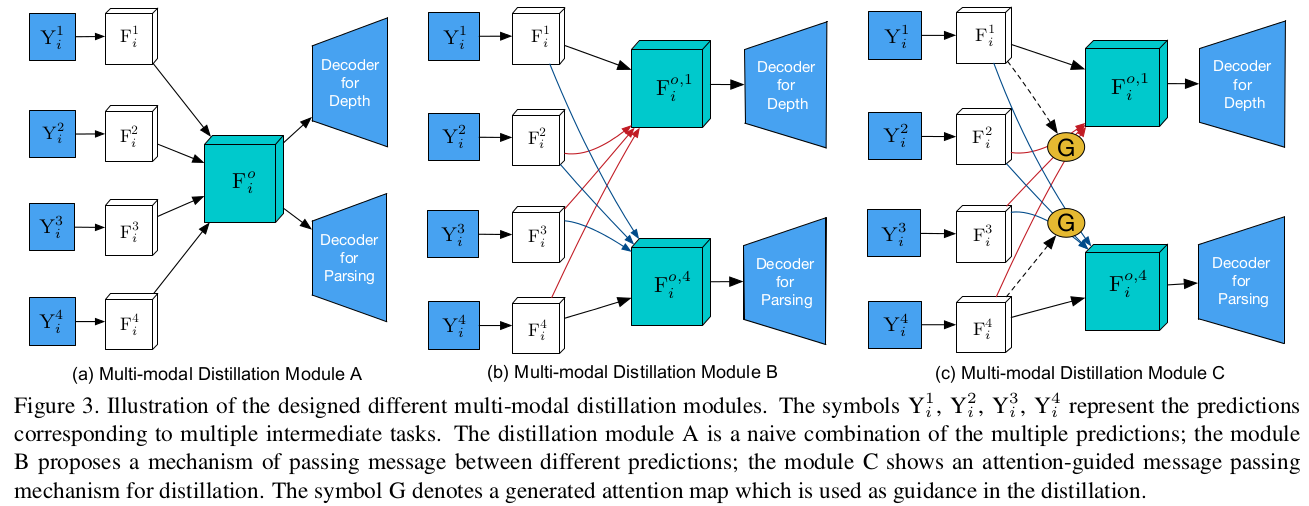
\includegraphics[width=0.75\textwidth]{DLTips/ThreeDistillationModules1.png}
\caption{三种不同的Distillation Module}
\label{ThreeDistillationModules1}
\end{figure}

\item Distillation loss function\cite{Mehta2018OD200}

利用Distillation帮助将Teacher Network(精度更高)的知识迁移到的Student Network.

\end{itemize}

\subsection{Knowledge Distillation}

\subsubsection{什么是Distilling the knowledge}

一句话总结,就是用teacher network的输出作为soft label来训练一个student network.

\subsubsection{Disilling the knowledge in a Neural Network}

\begin{displaymath}
q_i = \frac{exp(z_i/T)}{\sum_{j}exp(z_j/T)}
\end{displaymath}

其实就是一个Softmax,值得注意的是$T$是Temperature,$T$越大,概率分布就越Soft。在训练Student Network时,该概率分布就是Student Network的soft label.

Student Network 的训练策略:
\begin{itemize}
\item 先用Teacher Network的概率分布训练
\item 再用Real Label训练
\end{itemize}

\subsection{Recurrent Knowledge Distillation \cite{Silvia2018Recurrent}}

\section{光流估计中的Average end-point error}

貌似就是类似于均方误差类似。具体定义还没查到。

\section{CNN中的卷及方式汇总}

参考文献:\href{https://zhuanlan.zhihu.com/p/29367273}{CNN中的卷积方式2017.9-知乎}

\subsection{Inception}

\begin{figure}[!htbp]
\centering
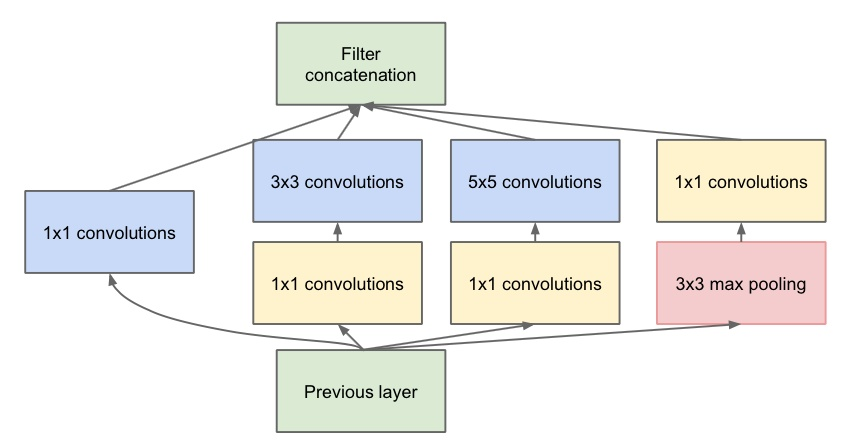
\includegraphics[width=0.9\textwidth]{DLTips/Inception0.jpg}
\caption{Inception卷积结构}
\label{Inception0}
\end{figure}
如图\ref{Inception0}所示。
主要思想是,融合Network in Network的思想来增加隐层提升非线性表达的思想。先用1*1的卷积映射到隐空间,再在隐空间做卷积操作。同时考虑多尺度,在单层Inception中,用多个大小不同的卷积核做卷积,然后把结果Concat起来。

代表模型:
\begin{itemize}
\item Inception-V1

就是把图\ref{Inception0}中的结构进行Stack,GoogLeNet?

\item Inception-V2

加入了Batch Normalization正则,去除了5*5卷积,用两个3*3卷积代替

\item Inception-V3

7 × 7卷积被拆分成7 * 1 + 1 * 7, 可分离卷积?

\item Inception-V4

加入了残差结构。

\end{itemize}

\subsection{空洞卷积, Dilation}

Dilation卷积,通常译作空洞卷积或者卷积核膨胀操作,它是解决pixel-wise输出模型的一种常用的卷积方式。一种普遍的认识是,pooling下采样操作导致的信息丢失是不可逆的,通常的分类识别模型,只需要预测每一类的概率,所以我们不需要考虑pooling会导致损失图像细节信息的问题,但是做像素级的预测时(譬如语义分割),就要考虑到这个问题了。

所以就要有一种卷积代替pooling的作用(成倍的增加感受野),而空洞卷积就是为了做这个的。通过卷积核插“0”的方式,它可以比普通的卷积获得更大的感受野。

所以,本意是为了增加感受野。

应用:
\begin{itemize}
\item FCN
\item WaveNet
\end{itemize}

\subsection{深度可分离卷积, Depthwise Separable Convolution}

是Incepion的延续。

\begin{figure}[!htbp]
\centering
\subfigure[简化的Inception]{\label{Inception1}
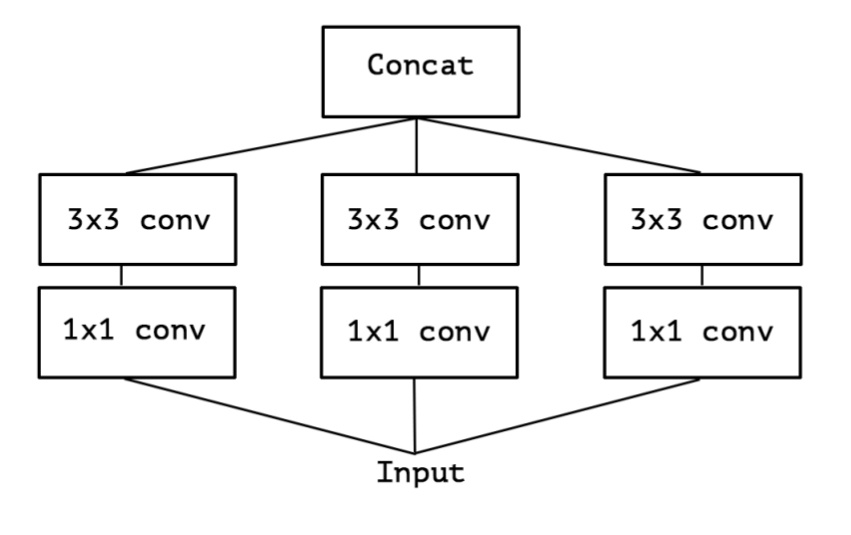
\includegraphics[width=0.95\textwidth]{DLTips/Inception1.jpg}}
\\
\subfigure[Depthwise Separable Convolution的示意图, 可以看出来,与Inception很像。]{\label{DepthwiseSeparable0}
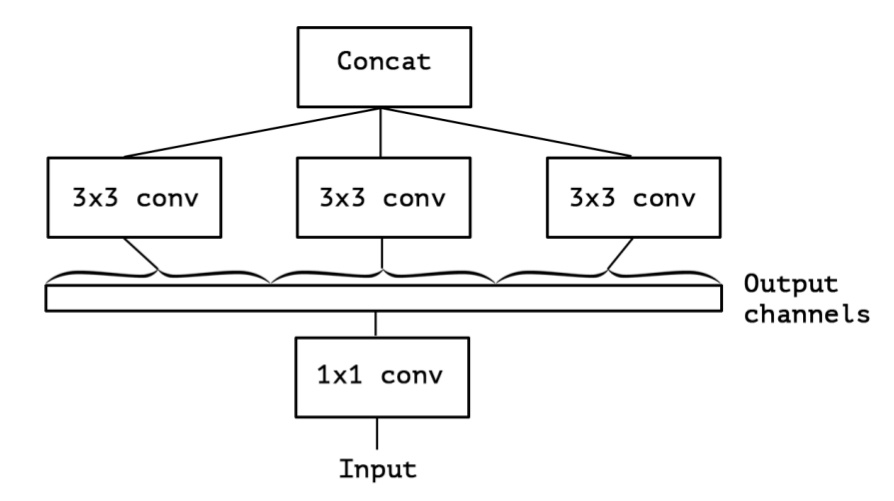
\includegraphics[width=0.95\textwidth]{DLTips/DepthwiseSeparable0.jpg}}
\caption{Inception结构与Depthwise Separable Convolution结构对比}
\label{InceptionAndDepthwise0}
\end{figure}

如图\ref{InceptionAndDepthwise0}所示,我们又可以看做,把一整个输入做1*1卷积,然后切成三段,分别3*3卷积后相连。注意的是,在三个不同的卷积时,是对Channel进行分组进行3*3卷积。

OK,现在我们想,如果不是分成三段,而是分成5段或者更多,那模型的表达能力是不是更强呢?于是我们就切更多段,切到不能再切了,正好是Output channels的数量(极限版本, 图\ref{DepthwiseSeparable1}):

\begin{figure}[!htbp]
\centering
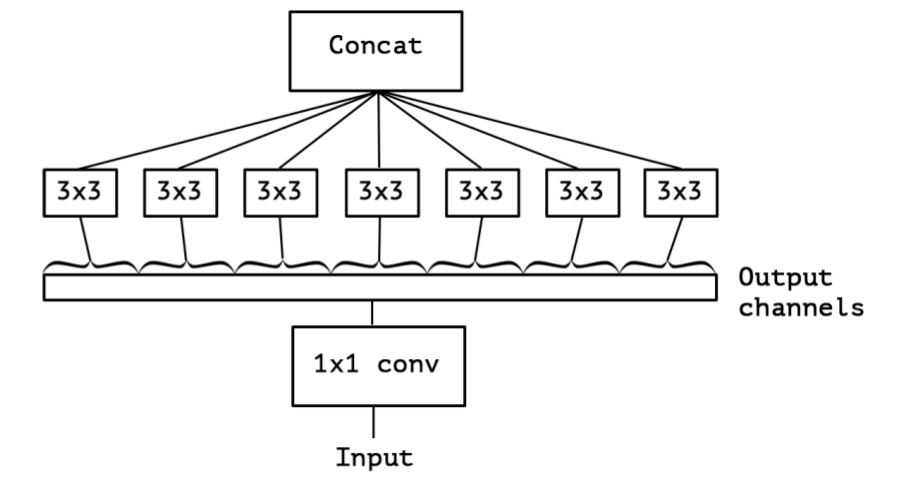
\includegraphics[width=0.75\textwidth]{DLTips/DepthwiseSeparable1.jpg}
\caption{Channel分组的极限版本}
\label{DepthwiseSeparable1}
\end{figure}

于是,就有了深度卷积(depthwise convolution),深度卷积是对输入的每一个channel独立的用对应channel的所有卷积核去卷积,假设卷积核的shape是[filter\_height, filter\_width, in\_channels, channel\_multiplier],那么每个in\_channel会输出channel\_multiplier那么多个通道,最后的feature map就会有in\_channels * channel\_multiplier个通道了。反观普通的卷积,输出的feature map一般就只有channel\_multiplier那么多个通道。

也就是说,对于每一个Channel, 都用不同的多个卷积核进行卷积,具体的是Channel\_multiplier个不同的卷积核。

既然叫深度可分离卷积,光做depthwise convolution肯定是不够的,原文在深度卷积后面又加了pointwise convolution,这个pointwise convolution就是1*1的卷积,可以看做是对那么多分离的通道做了个融合。

这两个过程合起来,就称为Depthwise Separable Convolution了。

应用:
\begin{itemize}
\item Xception
\end{itemize}

\subsection{可变性卷积}

可形变卷积的思想很巧妙:它认为规则形状的卷积核(比如一般用的正方形3*3卷积)可能会限制特征的提取,如果赋予卷积核形变的特性,让网络根据label反传下来的误差自动的调整卷积核的形状,适应网络重点关注的感兴趣的区域,就可以提取更好的特征。

如图\ref{DeformableConv0}:网络会根据原位置(a),学习一个offset偏移量,得到新的卷积核(b)(c)(d),那么一些特殊情况就会成为这个更泛化的模型的特例,例如图(c)表示从不同尺度物体的识别,图(d)表示旋转物体的识别。

\begin{figure}[!htbp]
\centering
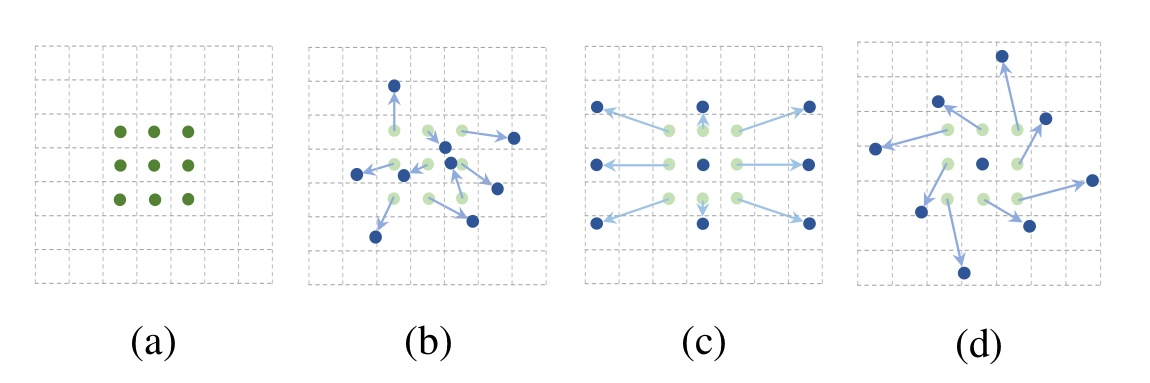
\includegraphics[width=0.95\textwidth]{DLTips/DeformableConv0.jpg}
\caption{Deformable Convolution示意图}
\label{DeformableConv0}
\end{figure}

具体实现如下。

%图\ref{DeformableConv1}中包含两处卷积,第一处是获取offsets的卷积,即我们对input feature map做卷积,得到一个输出(offset field),然后再在这个输出上取对应位置的一组值作为offsets。假设input feature map的shape为[batch,height,width,channels],我们指定输出通道变成两倍,卷积得到的offset field就是[batch,height,width,2×channels],为什么指定通道变成两倍呢?因为我们需要在这个offset field里面取一组卷积核的offsets,而一个offset肯定不能一个值就表示的,最少也要用两个值(x方向上的偏移和y方向上的偏移)所以,如果我们的卷积核是3*3,那意味着我们需要3*3个offsets,一共需要2*3*3个值,取完了这些值,就可以顺利使卷积核形变了。第二处就是使用变形的卷积核来卷积,这个比较常规。(这里还有一个用双线性插值的方法获取某一卷积形变后位置的输入的过程)

图\ref{DeformableConv1}中包含两处卷积。第一处是绿色的获取Offsets的卷积,即图中上方部分,这一处的输入是Input feature map,得到一个输出(Offset Feild), 然后再在这个输出上取一个卷积核大小的切片,作为卷积核对应位置的Offset。若Input Feature的尺寸为:$Batch, height, width, channels$, 其中,Batch表示批数, Channel表示输入的通道数,然后输出通道变为两倍,卷积得到的Offset Field就是$Batch, height, width, 2 *  channels$,那么为什么会翻倍呢, 也就是图中上半部分中的2N是什么意思呢?首先要确定一个卷积核的Offset,需要在不同的方向上单独确定,比如X, Y方向,所以就变成二倍了。在实际进行Deformable时,首先从Offset Field中对应位置上取一个对应卷积核的切片,如果卷积核是3 * 3,那么我们在两个方向都取一个3 * 3的切片,代表来年各个方向的Offset,然后就完成卷积核形变了。

第二处的卷积,是图中下方的表示,就是一个常规的卷积运算,只不过卷积核是经过上述Offset之后的变形卷积核。这里还有一个用双线性插值的方法来获取某一卷积形变后位置的输入的过程。

\begin{figure}[!htbp]
\centering
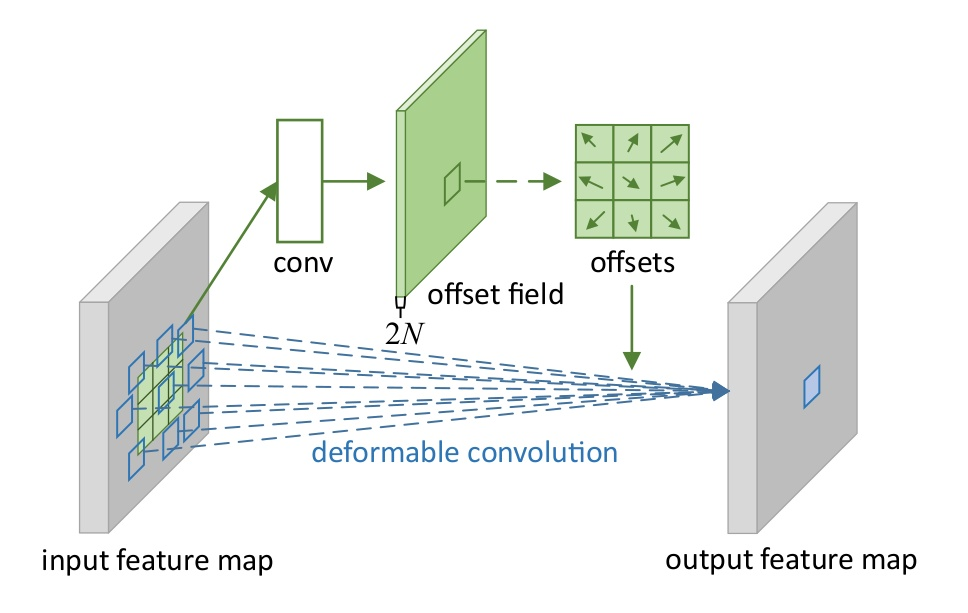
\includegraphics[width=0.95\textwidth]{DLTips/DeformableConv1.jpg}
\caption{Deformable Convolution的实现示意图}
\label{DeformableConv1}
\end{figure}

应用:
\begin{itemize}
\item Deformable Convolutional Networks
\end{itemize}

可能 会跟目标检测、跟踪相结合。

\subsection{特征重标定卷积}

在ImageNet2017比赛中,冠军模型SENet的核心模块,被称为"Squeeze-and-Excitation", 知乎的作者把它就先成为特征重标定卷积了。

和前面的不同,本文提出的算法的出发点在于改进特征为度,包括卷积核的数量等。现在一个卷积层中,还不是整个神经网络,有数以千计的卷积核,而且我们知道每一种卷积核对应提取一种特征,但得到这么多的特征,肯定有一些是更重要的,有一些是不那么重要的。所以本文的方法是通过学习方式来自动获取每个特征通道的重要程度,然后按照计算出来的重要程度去提升有用的特征并抑制对当前任务用处不大的特征。

\begin{figure}[!htbp]
\centering
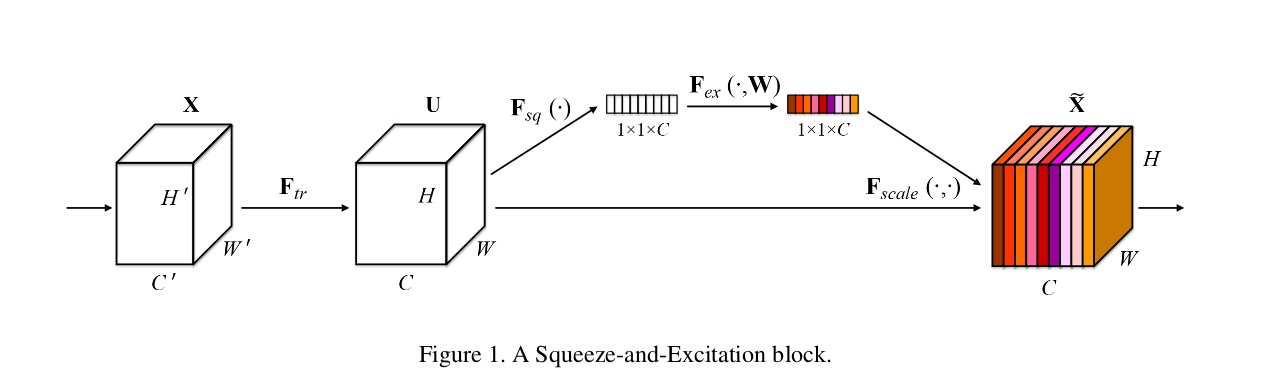
\includegraphics[width=0.9\textwidth]{DLTips/SENetConv0.jpg}
\caption{Squeeze-and-Excitation Block示意图}
\label{SENetConv0}
\end{figure}

虽然听上去很复杂,但实现起来却比较简单?步骤如下:
\begin{itemize}
\item 首先对输入$X$做常规的卷积$F_{tr}$,得到一个Output Feature Map ($U$),它的大小为$C, H, W$, 文章的作者认为,得到的这个Output是非常混乱的。
\item 为了得到这些Feature Maps(共$C$个)的重要程度,直接对这些Feature Map做一个Global Average Pooling\footnote{这里还涉及到一个额外的东西,如果你了解卷积,你就会发现一旦某一特征经常被激活,那么Global Average Pooling计算出来的值会比较大,说明它对结果的影响也比较大,反之越小的值,对结果的影响就越小。}, 然后就得到一个长度为$C$的向量,注意是向量了! 在图\ref{SENetConv0}中表现就是由$U$经操作$F_{sq}(\cdot)$得到$1 \times 1 \times C$的过程。

\item 然后我们对这个向量加两个FC层,做非线性映射,这俩FC层的参数,也就是网络需要额外学习的参数。对应图中$F_{ex}(\cdot, W)$操作。

\item 最后输出的向量,我们可以看做特征的重要性程度,然后与feature map对应channel相乘就得到特征有序的feature map了。对应图中$F_{scale}(\cdot, \cdot)$操作。
\end{itemize}

应用:
\begin{itemize}
\item Squeeze-and-Excitation Networks
\item 另外它还可以和几个主流网络结构结合起来一起用,比如Inception和Res。图\ref{SENetConv1}所示。
\end{itemize}

\begin{figure}[!htbp]
\centering
\subfigure[SE-Inception Module]{\label{SEInception0}
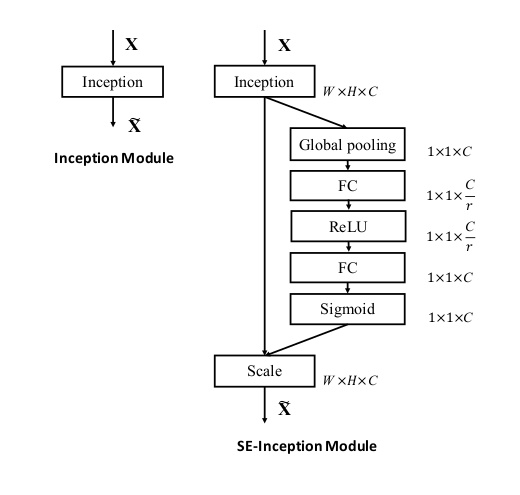
\includegraphics[width=0.45\textwidth]{DLTips/SEInception0.jpg}
}
\:
\subfigure[SE-ResNet Module]{\label{SEResNet0}
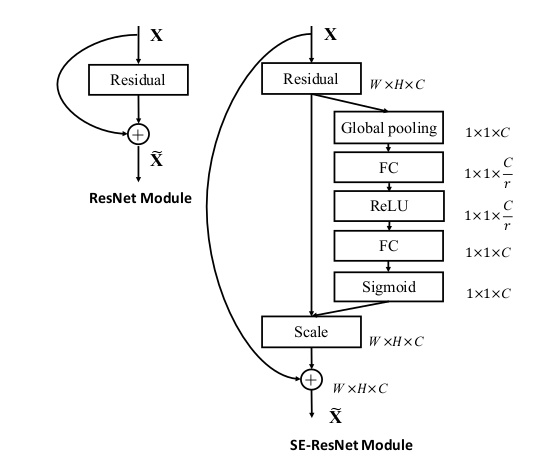
\includegraphics[width=0.45\textwidth]{DLTips/SEResNet0}
}
\caption{SENet与Inception以及ResNet结合的示意图}
\label{SENetConv1}
\end{figure}

\subsection{小结-比较}

图\ref{Conv0}是对上面提到的不同的卷及类型的一个比较与总结。

\begin{figure}
\centering
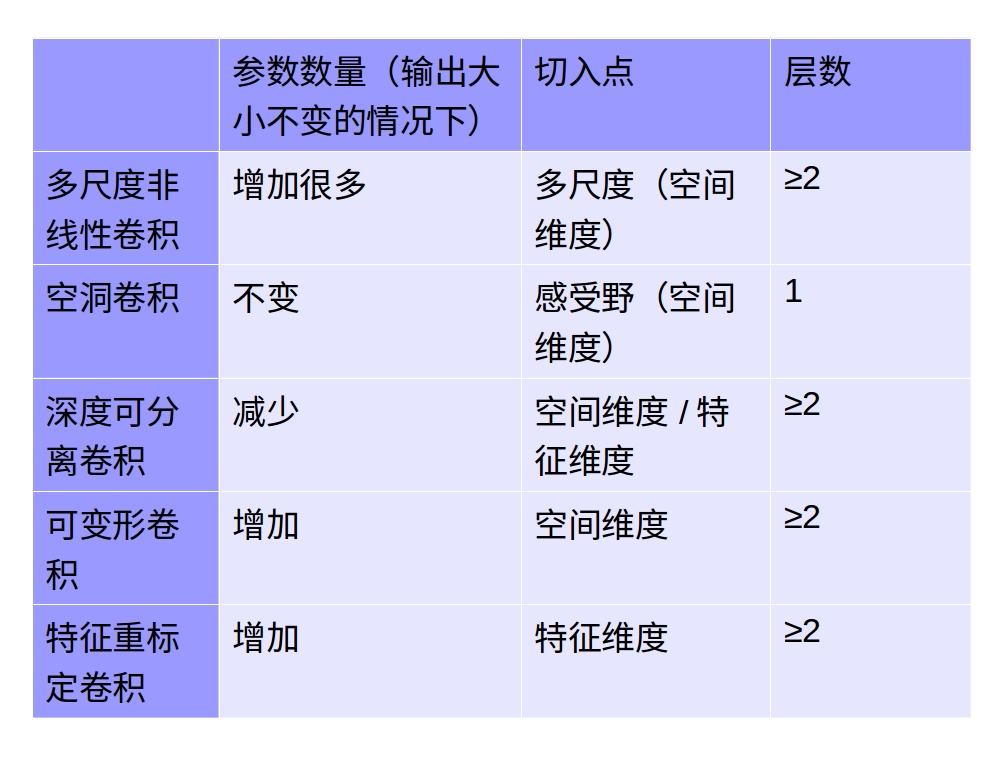
\includegraphics[width=0.75\textwidth]{DLTips/Conv0.jpg}
\caption{不同卷积策略的比较}
\label{Conv0}
\end{figure}

我们把图像(height,width)作为空间维度,把channels做为特征维度。

\section{全连接与卷积的异同}
全连接:Fully Connected

注意这里与FCN中的FC不同,FCN里面的FC是Fully Convolution,所以还是卷积操作,所以才有用Fully Convolution代替Fully Connected之说。

Fully Connected的作用是什么?其本质上还是一个卷积运算,只不过输入卷积核的大小跟最后一层Feature Map的大小一致, 所以得到的结果是一个标量。其实就是对前面CNN网络提取的特征进行变换,对这些Feature maps进行组合,得到目标类的一个代表值,输入Sigmoid函数进行计算,得到分类结果。但这种方式参数非常多,因为在实现Fully Connected时需要根据最后一层Feature Map的大小来确定计算的卷积核,这也导致了它需要解决不同输入大小时候的数据问题。

一个简单的例子,输入是$228 * 228 * 3$,然后最后一层Feature Map的维度是$7 * 7 * 512$,即,共包含512个Feature Maps,每一个Feature Map的大小是$7 * 7$,那么全连接层需要这样设计,假设我们想要输出1024个分类,那么全连接的参数的数量就是:
$7 * 7 * 512 * 1024$,所以参数非常多!另一方面,如果输入不是$228 * 228 * 3$而是$456 * 456 * 3$那么,得到的最后一层Feature map的大小也不是$7 * 7 * 512$,现在而是$14 * 14 * 512$,那么全连接也需要改变,变成$14 * 14 * 512 * 1024$, 这样非常不灵活。

因为参数实在太多,所以现在在最后为了得到Sigmoid函数的输入(标量),都选择使用Global Average Pooling来代替全连接。Global Average Pooling也就是说用一个Feature Map的平均值作为Sigmoid输入,输出为类别信息。

不过,也有研究人员表明,全连接层有助于在微调(Fine-tune)过程中进行知识迁移,尤其源领域与目标领域很不一样的时候,更是如此。

\section{Pooling}

\subsubsection{Global Average Pooling}

就是对一个Feature Map进行加和求平均值。具体的应用可参考上一小节。

\subsubsection{Unpooling}

而上池化的实现主要在于池化时记住输出值的位置,在上池化时再将这个值填回原来的位置,其他位置填0即OK。(参考:SegNet, DeconvNet)

\begin{figure}[!hbtp]
\centering
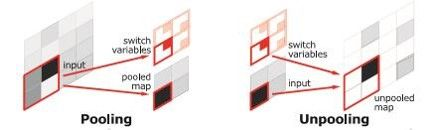
\includegraphics[width=0.75\textwidth]{DLTips/Unpooling0.png}
\caption{Unpooling示意图}
\label{Unpooling0}
\end{figure}

图\ref{Unpooling0}可以认为额外的\verb|switch variables|实现了保存Pooling过程中的位置。

In the convnet, the max pooling operation is non-invertible, however we can obtain an approximate inverse by recording the locations of the maxima within each pooling region in a set of switch variables. In the deconvnet, the unpooling operation uses these switches to place the reconstructions from the layer above into appropriate locations, preserving the structure of the stimulus.

也就是说用一组开关变量保存最大值在Pooling Region中的位置。

参考文献: \href{https://www.quora.com/What-is-the-difference-between-Deconvolution-Upsampling-Unpooling-and-Convolutional-Sparse-Coding}{Quora Answer}

\section{Local Response Normalization}

Reference: \href{https://prateekvjoshi.com/2016/04/05/what-is-local-response-normalization-in-convolutional-neural-networks/}{What is LRN}

为什么需要设置Normalization Layers?
Anyway, the reason we may want to have normalization layers in our CNN is that we want to have some kind of inhibition scheme. 这个Inhibition Scheme是什么意思。

侧边抑制:ateral inhibition。 一个激活的神经会抑制旁边神经的激活。

\subsubsection{到底什么是LRN}

Local Response Normalization (LRN) layer implements the lateral inhibition we were talking about in the previous section. This layer is useful when we are dealing with ReLU neurons. Why is that? Because ReLU neurons have unbounded activations and we need LRN to normalize that. We want to detect high frequency features with a large response. If we normalize around the local neighborhood of the excited neuron, it becomes even more sensitive as compared to its neighbors.

At the same time, it will dampen(抑制) the responses that are uniformly large in any given local neighborhood(值普遍很大的局部). If all the values are large, then normalizing those values will diminish all of them. So basically we want to encourage some kind of inhibition and boost the neurons with relatively larger activations. 

\subsubsection{如何实现LRN}

There are two types of normalizations available in Caffe. You can either normalize within the same channel or you can normalize across channels. Both these methods tend to amplify the excited neuron while dampening the surrounding neurons. When you are normalizing within the same channel, it’s just like considering a 2D neighborhood of dimension N x N, where N is the size of the normalization window. You normalize this window using the values in this neighborhood. If you are normalizing across channels, you will consider a neighborhood along the third dimension but at a single location. You need to consider an area of shape N x 1 x 1. Here 1 x 1 refers to a single value in a 2D matrix and N refers to the normalization size.

在 AlexNet 中Normalized的计算公式如下:

\begin{displaymath}
b_{x, y}^i = a_{x, y}^i / \left( k + \alpha \sum_{j = \max(0, i - n/2)}^{\min(N-1, i + n/2)(a_{x, y}^j)^2} \right)
\end{displaymath}

其中, $a_{x, y}^i, b_{x, y}^i$分别是输入的激活值,输出的Normalized的值。

\section{CNN中感受野的计算}

参考文献:

[1] \href{https://blog.csdn.net/kuaitoukid/article/details/46829355}{CNN中感受野的计算-CSDN}

[2] \href{https://www.cnblogs.com/objectDetect/p/5947169.html}{CNn中感受野的计算-博客园}

感受野(receptive field)是怎样一个东西呢,从CNN可视化的角度来讲,就是输出featuremap某个节点的响应对应的输入图像的区域就是感受野。

比如我们第一层是一个3*3的卷积核,那么我们经过这个卷积核得到的featuremap中的每个节点都源自这个3*3的卷积核与原图像中3*3的区域做卷积,那么我们就称这个featuremap的节点感受野大小为3*3

如果再经过pooling层,假定卷积层的stride是1,pooling层大小2*2,stride是2,那么pooling层节点的感受野就是4*4

有几点需要注意的是,padding并不影响感受野,stride只影响下一层featuremap的感受野,size影响的是该层的感受野。

具体计算时,需要:
\begin{itemize}
\item 第一层卷积层的输出特征像素的感受野的大小就是滤波器的大小
\item 深层卷积层的感受野大小和它之前的所有层的滤波器大小和步长有关系
\item 计算感受野大小时,忽略图像边缘的影响,即不考虑Padding的大小。
\end{itemize}

关于感受野的计算,多采用Top to Down的方式,即最先计算最深层的前一层的感受野,然后逐渐传递到第一层,使用的公式如下:
\begin{enumerate}
\item RF = 1   // 待计算的Feature Map的感受野大小
\item For layer in (top layer to down layer):
\item      RF = ((RF - 1) * stride) + fsize
\end{enumerate}

stride 表示卷积的步长; fsize表示卷积层滤波器的大小。

\subsubsection{具体的例子}

%\begin{table}
\begin{tabular}{ccc}
\toprule
type & size & stride \\
\midrule
conv1 & 3 & 2 \\
pool1 & 2 & 2 \\
conv2 & 3 & 1 \\
pool2 & 2 & 2 \\
conv3 & 3 & 1 \\
conv4 & 3 & 1 \\
pool3 & 2 & 2 \\
\bottomrule
\end{tabular}
%\end{table}

pool3的一个输出对应pool3的输入大小为2*2

感受野计算如下:

依次类推,对应conv4的输入为4*4,因为2*2的每个角加一个3*3的卷积核,就成了4*4,当然这是在stride=1的情况下才成立的,但是一般都是stride=1,不然也不合理

对应conv3的输入为6*6

对应pool2的输入为12*12

对应conv2的输入为14*14

对应pool1的输入为28*28

对应conv1的输入为30*30

所以pool3的感受野大小就是30*30

\subsubsection{Stride的计算}

每一个卷积层有一个Strides的概念,这个Strides就是之前所有层Stride的乘积。即
\begin{displaymath}
strids(i) = stride(1) * stride(2) * stride(3) * \ldots * stride(i - 1)
\end{displaymath}

\subsubsection{专业的计算}

参考文献:\href{https://zhuanlan.zhihu.com/p/26663577}{卷积神经网络中的感受野计算(译)-知乎}, \href{https://medium.com/mlreview/a-guide-to-receptive-field-arithmetic-for-convolutional-neural-networks-e0f514068807}{原文-英语}





\section{待续}













